\begin{savequote}[45mm]
\ascii{Any fool can write code that a computer can understand. Good programmers write code that humans can understand.}
\qauthor{\ascii{- Martin Flower}}
\end{savequote}

\chapter{Saver} 
\label{ch:saver}

\section{Saver}

\begin{content}

在长期的训练任务过程中,为了实现任务的高可用性,\tf{}会周期性地执行断点检查(\ascii{Checkpoint})。

\code{Saver}是实现断点检查功能的基础设施,它会将所有的训练参数持久化在文件系统中;当需要恢复训练时,可以载从文件系统中恢复计算图,及其训练参数的值。也就是说,\code{Saver}承担如下两个方面的职责:

\begin{enum}
  \eitem{\code{save}: 将训练参数的当前值持久化到断点文件中;}
  \eitem{\code{restore}: 从断点文件中恢复训练参数的值。} 
\end{enum}

\subsection{使用方法}

例如,存在一个简单的计算图,包含两个训练参数。首先,执行初始化后,将其结果持久化到文件系统中。

\begin{leftbar}
\begin{python}
# construct graph
v1 = tf.Variable([0], name='v1')
v2 = tf.Variable([0], name='v2')

# run graph
with tf.Session() as sess:
  sess.run(tf.global_variables_initializer())
  saver = tf.train.Saver()
  saver.save(sess, 'ckp')
\end{python}
\end{leftbar}

随后,可以根据断点文件存储的位置恢复模型。

\begin{leftbar}
\begin{python}
with tf.Session() as sess:
  saver = tf.import_meta_graph('ckp.meta')
  saver.restore(sess, 'ckp')
\end{python}
\end{leftbar}

\subsection{文件功能}

当执行\code{Saver.save}操作之后,在文件系统中生成如下文件:

\begin{leftbar}
\begin{python}
├── checkpoint
├── ckp.data-00000-of-00001
├── ckp.index
├── ckp.meta
\end{python}
\end{leftbar}

\subsubsection{索引文件}

索引(\ascii{index})文件保存了一个不可变表(\code{tensorflow::table::Table})的数据;其中,关键字为\ascii{Tensor}的名称,其值描述该\ascii{Tensor}的元数据信息,包括该\ascii{Tensor}存储在哪个数据(\ascii{data})文件中,及其在该数据文件中的偏移,及其校验和等信息。

\subsubsection{数据文件}

数据(\ascii{data})文件记录了所有变量\ascii{(Variable)}的值。当\code{restore}某个变量时,首先从索引文件中找到相应变量在哪个数据文件,然后根据索引直接获取变量的值,从而实现变量数据的恢复。

\subsubsection{元文件}

元文件(\ascii{meta})中保存了\code{MetaGraphDef}的持久化数据,它包括\code{GraphDef, SaverDef}等元数据。

将描述计算图的元数据与存储变量值的数据文件相分离,实现了静态的图结构与动态的数据表示的分离。因此,在恢复\ascii{(Restore)}时,先调用\code{tf.import\_meta\_graph}先将\code{GraphDef}恢复出来,然后再恢复\code{SaverDef},从而恢复了描述静态图结构的\code{Graph}对象,及其用于恢复变量值的\code{Saver}对象,最后使用\code{Saver.restore}恢复所有变量的值。

这也是在上例中,在调用\code{Saver.restore}之前,得先调用\code{tf.import\_meta\_graph}的真正原因;否则,缺失计算图的实例,就无法谈及恢复数据到图实例中了。

\subsubsection{状态文件}

\ascii{Checkpoint}文件会记录最近一次的断点文件(\ascii{Checkpoint File})的前缀,根据前缀可以找对对应的索引和数据文件。当调用\code{tf.train.latest\_checkpoint},可以快速找到最近一次的断点文件。


此外,\ascii{Checkpoint}文件也记录了所有的断点文件列表,并且文件列表按照由旧至新的时间依次排序。当训练任务时间周期非常长,断点检查将持续进行,必将导致磁盘空间被耗尽。为了避免这个问题,存在两种基本的方法:

\begin{enum}
  \eitem{\code{max\_to\_keep}: 配置最近有效文件的最大数目,当新的断点文件生成时,且文件数目超过\code{max\_to\_keep},则删除最旧的断点文件;其中,\code{max\_to\_keep}默认值为\ascii{5};}
  \eitem{\code{keep\_checkpoint\_every\_n\_hours}: 在训练过程中每\code{n}小时做一次断点检查,保证只有一个断点文件;其中,该选项默认是关闭的。} 
\end{enum}

由于\ascii{Checkpoint}文件也记录了断点文件列表,并且文件列表按照由旧至新的时间依次排序。根据上述策略删除陈旧的断点文件将变得极其简单有效。

\subsection{模型}

\subsubsection{持久化模型}

为了实现持久化的功能,\code{Saver}在构造时在计算图中插入\code{SaveV2},及其关联的\ascii{OP}。其中,\code{file\_name}为一个\ascii{Const}的\ascii{OP},指定断点文件的名称;\code{tensor\_names}也是一个\ascii{Const}的\ascii{OP},用于指定训练参数的\ascii{Tensor}名称列表。

\begin{figure}[!htbp]
\centering
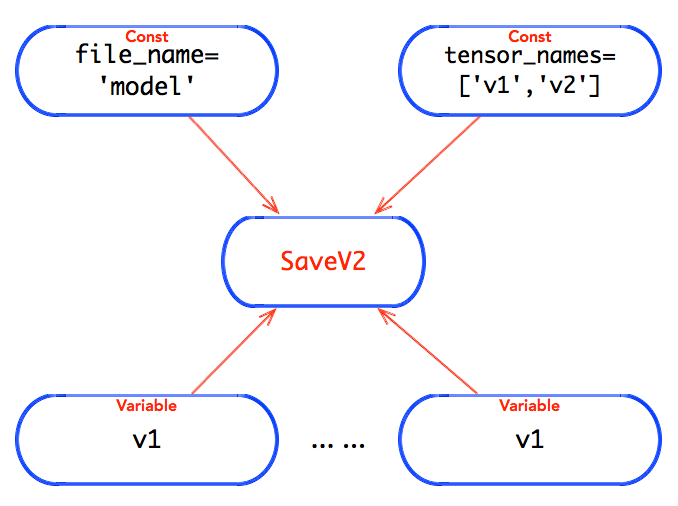
\includegraphics[width=0.5\textwidth]{figures/py-saver-save-model.png}
\caption{Saver:持久化模型}
 \label{fig:py-saver-save-model}
\end{figure}

\subsubsection{恢复模型}

同样地,为了实现恢复功能,\code{Saver}在构造期,为每个训练参数,插入了一个\code{RestoreV2},及其关联的\ascii{OP}。其中,包括从断点文件中恢复参数默认值的初始化器\ascii{(Initializer)},其本质是一个\code{Assign}的\ascii{OP}。 

另外,\code{file\_name}为一个\ascii{Const}的\ascii{OP},指定断点文件的名称;\code{tensor\_names}也是一个\ascii{Const}的\ascii{OP},用于指定训练参数的\ascii{Tensor}名称列表,其长度为\ascii{1}。

\begin{figure}[!htbp]
\centering
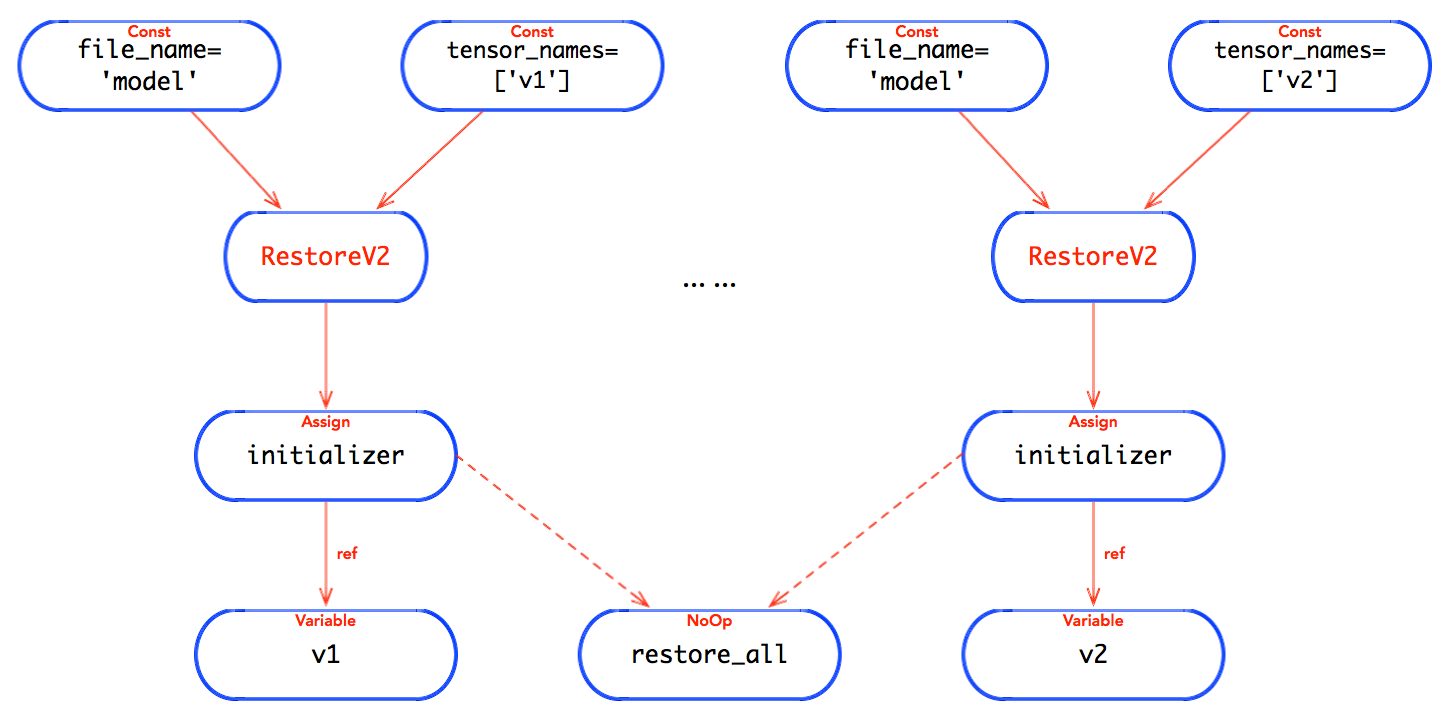
\includegraphics[width=0.9\textwidth]{figures/py-saver-restore-model.png}
\caption{Saver:恢复模型}
 \label{fig:py-saver-restore-model}
\end{figure}

\end{content}
